\chapter*{O prohlížeči}
\addcontentsline{toc}{chapter}{O prohlížeči}
\section*{Úvod}
\addcontentsline{toc}{section}{Zadání}
V roce 2009 byl v rámci spolupráce s IKEM\footnote{Institut Klinické a Experimentální medicíny} zahájen vývoj prohlížeče snímků z magnetické resonance. Prohlížeč by měl sloužit k výzkumným účelům. Program by měl otevírat speciální formát snímků DICOM\footnote{DICOM je standard pro ukládání medicínských dat.} a dále umožňovat jednoduché úpravy snímku: zvětšování, zmenšování, změna jasu a kontrastu. Od ostatních prohlížečů se pak má odlišovat tím, že bude umožňovat otevírání více lékařských studií na jedné pracovní ploše ve zcela volném uspořádání. Tato funkce odborníkům z IKEM značně scházela u volně dostupných prohlížečů (lze pak porovnávat různé patologické stavy onemocnění). Další funkcí, která není zcela běžná, mělo být to, že DicomPresenter bude umožňovat zaznamenání práce uživatele se snímky a výsledek pak exportovat do videa (video pak lze použít při prezentacích).

Při vývoji aplikace byl kladen důraz na jeho plynulý běh. Práce \cite{neskudla}, v rámci které byl vývoj prohlížeče zahájen, tedy hledala odpověď na otázku, zda je možné využít pro tuto aplikaci vlastnosti moderních grafických akcelerátorů. Renderování grafického výstupu aplikace grafickou kartou pomocí OpenGL, namísto renderování na procesoru, mělo výrazně přispět ke zcela plynulému chodu aplikace.

Jakou součást práce \cite{neskudla} byla naprogramována první verze prohlížeče. Na základě této verze mělo být rozhodnuto, jakým směrem se prohlížeč bude dále vyvíjet. Vývoj pokračoval v práci \cite{flaska}. V práci byly odstraněny některé závažné chyby, kvůli kterým program nefungoval. Dále byl jako součást práce naprogramován skript Cmake, který měl umožňovat překlad programu na dalších počítačích. V práci byl vývoj skriptu orientován na OS Linux. Aplikace tak byla nově přeložitelná na Linuxových systémech.


\section*{Popis uživatelského rozhraní DicomPresenteru}
\addcontentsline{toc}{section}{Popis uživatelského rozhraní DicomPresenteru}
\begin{figure}
	\begin{center}
	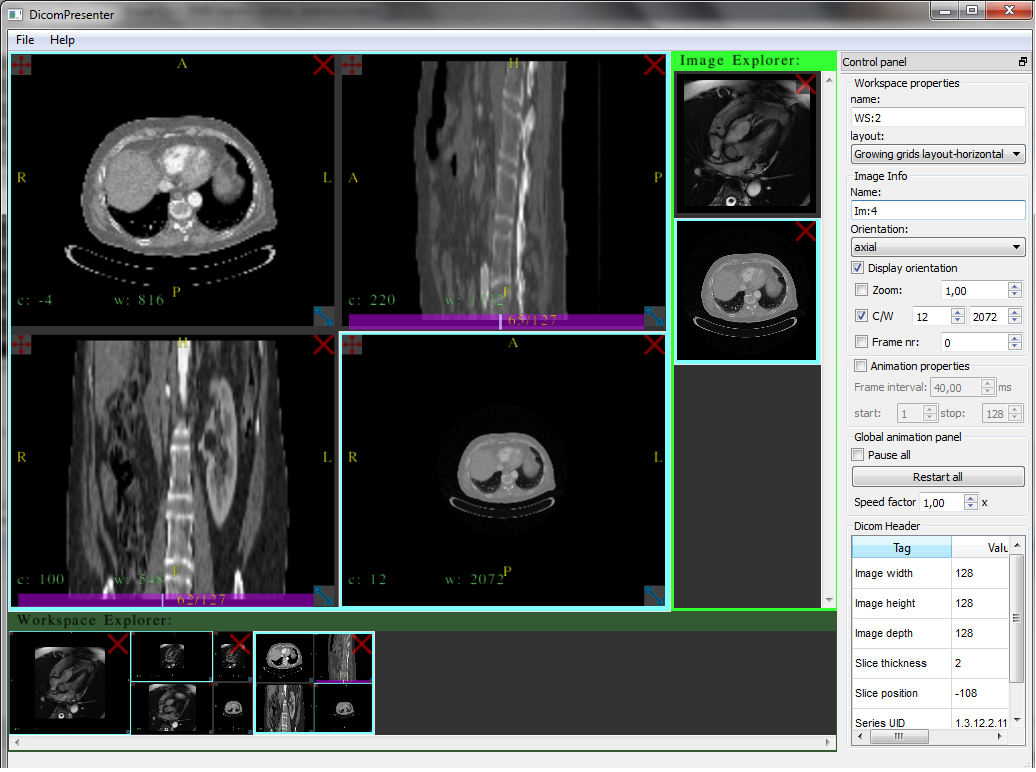
\includegraphics[width=130mm]{Text/IMG/04_GUI_Screenshot.png}
	\end{center}
	\caption{Rozhraní programu Dicom Presenter}
	\label{screenshot}
\end{figure}
Okno programu je rozdělené na dvě základní části (viz obrázek~\ref{screenshot}). V pravé části okna je panel nastavení, kde se dají měnit vlastnosti snímků. Zbytek okna zabírá tzv. vykreslovací okno - to je samotné rozděleno na tři části. Ve spodní nalezneme seznam používaných pracovních ploch, v pravé seznam otevřených snímků. Samotná pracovní plocha je pak promítána na největší, prostřední část okna.

Uživatel při práci s programem může mít otevřeno více pracovních ploch se snímky, mezi nimi se pak přepíná pomocí jejich seznamu. Snímky na pracovní ploše je možné rozmisťovat téměř libovolně. Jejich pozice a velikost na pracovní ploše se dá přizpůsobit pomocí tlačítek na ploše.

Jednotlivé snímky je možné posunovat přibližovat a oddalovat a dále měnit jejich jas a kontrast. Kolečkem na myši pak lze posunovat řez v rámci celého trojrozměrného snímku (kolmo k rovině promítání).

Práci se snímky na pracovní ploše je možné zachytit do animace a tu pak exportovat jako video (nastavením v ovládacím panelu a pak exportem skrze File-> Save animation).

\chapter*{Cíl práce}
\addcontentsline{toc}{chapter}{Cíl práce}
Zadání tohoto výzkumného úkolu bylo shrnuto ve třech bodech, které reflektují problémy, které se s programem objevily a dále potřeby jak program upravit.

\begin{itemize}
\item Zajistěte bezchybný překlad a běh aplikace a její instalaci na počítačích ve středisku IKEM.
\item Prozkoumejte možnosti zjednodušení struktury programu (odstranění závislosti na některých knihovnách) za účelem dosažení snadné přenositelnosti.
\item V návaznosti na konzultace s kolegy v IKEM implementujte nové funkce podle jejich potřeb.
\end{itemize}

\section*{Zajištění bezchybného překladu aplikace}
\addcontentsline{toc}{section}{Zajištění bezchybného překladu aplikace}
Vývojová verze programu DicomPresenter bohužel nešla spustit na jiných počítačích, než na kterých byla programována. V práci \cite{flaska} se autor zabýval překladem aplikace na OS Linux, což výrazně pomohlo k pročištění zdrojového kódu. Nicméně ve středisku IKEM je potřeba provozovat aplikaci na počítačích vybavených Windows. Z tohoto důvodu bylo nutné, v první fázi práce na tomto VÚ, obstarat takový překlad aplikace, aby aplikace byla spustitelná na většině počítačů. V tomto dokonale posloužil skript Cmake, který byl napsán pro překlad programu na OS Linux a to jako součást práce \cite{flaska}. Cmake je vyvíjen jakožto multiplatformní nástroj pro překlad programů a tak se také osvědčil. 

Při překladu se dále objevily potíže, které vznikaly díky zapojení velkého počtu externích knihoven v programu, jednalo se o nekompatibilitu přeložených součástí programu - kód lze přeložit s různými verzemi standardních knihoven.

Poznatky získané při výše popsané práci na DicomPresenteru byly shrnuty a popsány v druhé kapitole této práce.

\section*{Zjednodušení programu}
\addcontentsline{toc}{section}{Zjednodušení programu}
Při zprovozňování DicomPresenteru na počítačích v IKEM a na počítačích s Windows obecně docházelo ke značným komplikacím plynoucím ze zapojení většího množství externích knihoven v programu. Problémy byly s nekompatibilitou pixel shaderu používajícího knihovnu Cg toolkit, problémy vznikaly při pokusech o překlad, kdy v programu byly navzájem nekompatibilně přeložené externí knihovny (viz předchozí bod) a nejhorším problémem s kompatibilitou byla nefunkčnost programu na počítačích se staršími grafickými kartami. Na základě těchto problémů byl ze strany školitele vznesen požadavak na studii toho, zda by bylo možné odstranit některé externí knihovny z programu, jmenovitě: Cg toolkit, OpenGL, plib.

Zapojení Cg toolkit v programu bylo učiněno na základě rozhodnutí autora v práci \cite{neskudla} a to z důvodu nedostatečné funkčnosti knihovny OpenGL pro implementaci změny jasu a kontrastu v programu. Knihovna OpenGL byla v programu využita k urychlení grafického výstupu a k zrychlení prováděných grafických operací.

Jak vyplývá z předchozích dvou odstavců, nutným požadavkem pro odstranění nadbytečných knihoven z kódu programu tak bylo:

\begin{itemize}
\item Zjistit, zda je možné realizovat grafické operace prováděné pomocí Cg toolkit pouze pomocí knihovny OpenGL.
\item Zjistit, jaký vliv by mělo případné odstranění knihovny OpenGL rychlost programu.
\end{itemize}


\section*{Implementace nových funkcí}
\addcontentsline{toc}{section}{Implementace nových funkcí}
Vedle samotného výzkumu, který by měl být základem této práce, je dále důležité posunout vývoj DicomPresenteru o krok dál, aby se program přiblížil ke stavu, kdy jej bude možné denně používat. Součástí práce na tomto VÚ tak bylo programování samotné aplikace. Vedle již zmíněné migrace z vývojové fáze na běžné počítače, to byly hlavně dva následující úkoly: V první řadě byla v programu implementována možnost multiplanární rekonstrukce třírozměrného nímku. Druhým úkolem pak bylo zjištění příčiny, proč se převážná většina volně dostupných Dicom snímků nechce v programu otevřít a odstranění této chyby. Užitečné zkušenosti, které byly získané při této práci, byly shrnuty v třetí kapitole této práce a měly by tak posloužit dalšímu studentovi, který se zapojí do vývoje DicomPresenteru, jako zdroj praktických poznatků.
